
\begin{figure}[htbp]
    \centering
    \hspace*{-0.15\textwidth}
    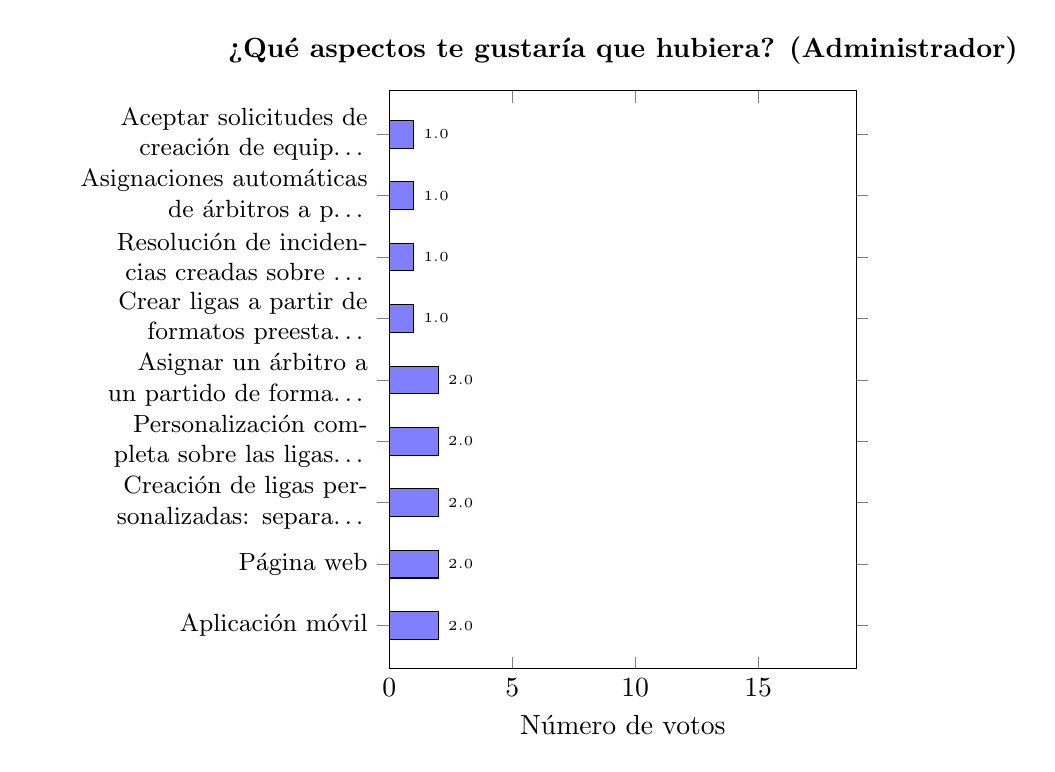
\begin{tikzpicture}
        \begin{axis}[
            title={\textbf{¿Qué aspectos te gustaría que hubiera? (Administrador)}},
            width=0.62*\textwidth,
            xbar,
            bar width=10pt,
            y=0.78cm,
            enlarge y limits={abs=0.55cm},
            xmin=0, xmax=19,
            xlabel={Número de votos},
            ytick={1,2,3,4,5,6,7,8,9},
            yticklabels={{Aplicación móvil}, {Página web}, {Creación de ligas personalizadas: separa\dots}, {Personalización completa sobre las ligas\dots}, {Asignar un árbitro a un partido de forma\dots}, {Crear ligas a partir de formatos preesta\dots}, {Resolución de incidencias creadas sobre \dots}, {Asignaciones automáticas de árbitros a p\dots}, {Aceptar solicitudes de creación de equip\dots}},
            yticklabel style={
                text width=4.2cm,
                align=right,
                font=\small
            },
            nodes near coords, 
            nodes near coords align={horizontal},
            every node near coord/.append style={
                font=\tiny,
                anchor=west,
                /pgf/number format/.cd, fixed, fixed zerofill, precision=1
            }
        ]
        \addplot[fill=blue!50] coordinates {
            (2, 1) (2, 2) (2, 3) (2, 4) (2, 5) (1, 6) (1, 7) (1, 8) (1, 9)
        };
        \end{axis}
    \end{tikzpicture}
    \label{fig:col_desired_functionalities_admin}
    \caption{Nuevas funcionalidades: Administrador}
\end{figure}

Vemos como los administradores buscan una mayor versatilidad y facilidad a la hora de poder gestionar la liga desde cualquier dispositivo. Una gestión amena que no genere fricción con el usuario.

\begin{figure}[htbp]
    \centering
    \hspace*{-0.15\textwidth}
    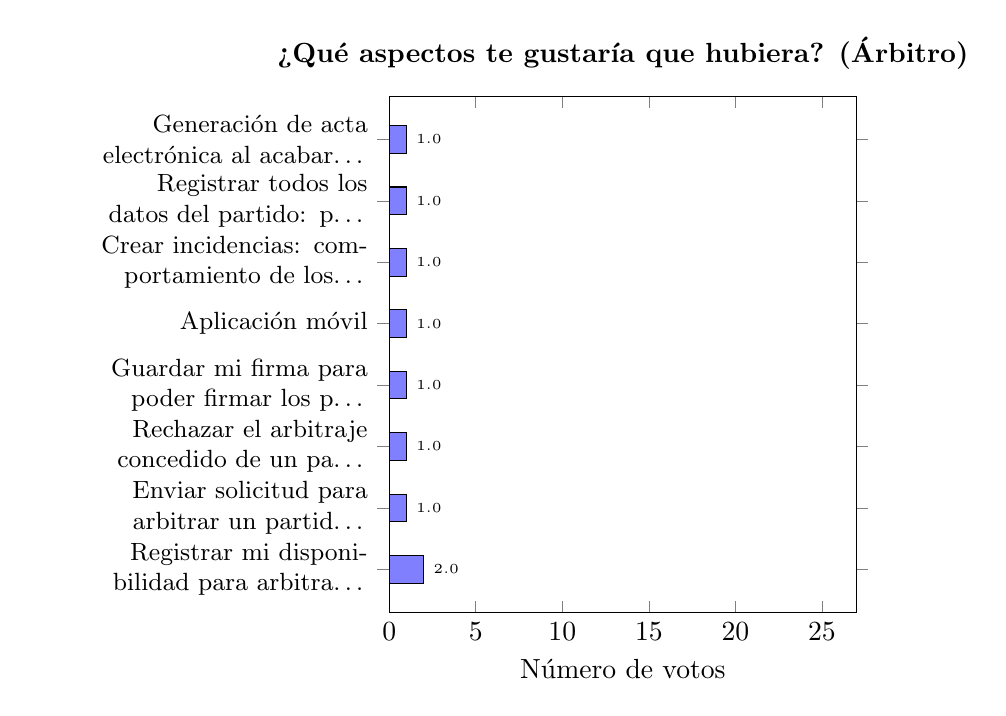
\begin{tikzpicture}
        \begin{axis}[
            title={\textbf{¿Qué aspectos te gustaría que hubiera? (Árbitro)}},
            width=0.62*\textwidth,
            xbar,
            bar width=10pt,
            y=0.78cm,
            enlarge y limits={abs=0.55cm},
            xmin=0, xmax=27,
            xlabel={Número de votos},
            ytick={1,2,3,4,5,6,7,8},
            yticklabels={{Registrar mi disponibilidad para arbitra\dots}, {Enviar solicitud para arbitrar un partid\dots}, {Rechazar el arbitraje concedido de un pa\dots}, {Guardar mi firma para poder firmar los p\dots}, {Aplicación móvil}, {Crear incidencias: comportamiento de los\dots}, {Registrar todos los datos del partido: p\dots}, {Generación de acta electrónica al acabar\dots}},
            yticklabel style={
                text width=4.2cm,
                align=right,
                font=\small
            },
            nodes near coords, 
            nodes near coords align={horizontal},
            every node near coord/.append style={
                font=\tiny,
                anchor=west,
                /pgf/number format/.cd, fixed, fixed zerofill, precision=1
            }
        ]
        \addplot[fill=blue!50] coordinates {
            (2, 1) (1, 2) (1, 3) (1, 4) (1, 5) (1, 6) (1, 7) (1, 8)
        };
        \end{axis}
    \end{tikzpicture}
    \label{fig:col_desired_functionalities_referee}
    \caption{Nuevas funcionalidades: Árbitro}
\end{figure}

Mientras que los árbitros se centran principalmente en que puedan especificar su disponibilidad y que el sistema actúe acorde.

\begin{figure}[htbp]
    \centering
    \hspace*{-0.15\textwidth}
    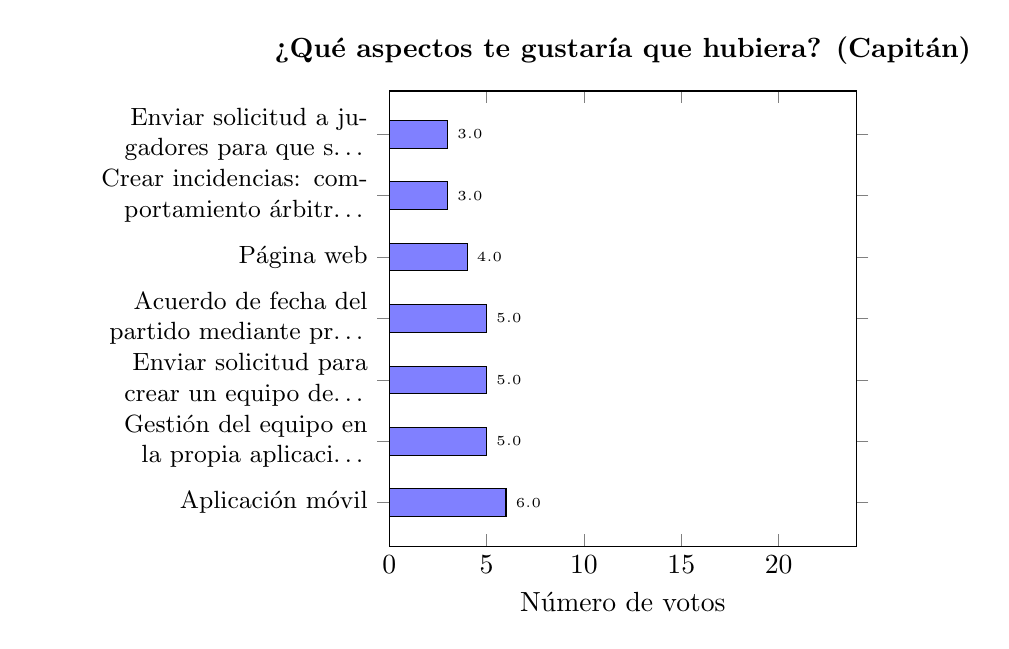
\begin{tikzpicture}
        \begin{axis}[
            title={\textbf{¿Qué aspectos te gustaría que hubiera? (Capitán)}},
            width=0.62*\textwidth,
            xbar,
            bar width=10pt,
            y=0.78cm,
            enlarge y limits={abs=0.55cm},
            xmin=0, xmax=24,
            xlabel={Número de votos},
            ytick={1,2,3,4,5,6,7},
            yticklabels={{Aplicación móvil}, {Gestión del equipo en la propia aplicaci\dots}, {Enviar solicitud para crear un equipo de\dots}, {Acuerdo de fecha del partido mediante pr\dots}, {Página web}, {Crear incidencias: comportamiento árbitr\dots}, {Enviar solicitud a jugadores para que s\dots}},
            yticklabel style={
                text width=4.2cm,
                align=right,
                font=\small
            },
            nodes near coords, 
            nodes near coords align={horizontal},
            every node near coord/.append style={
                font=\tiny,
                anchor=west,
                /pgf/number format/.cd, fixed, fixed zerofill, precision=1
            }
        ]
        \addplot[fill=blue!50] coordinates {
            (6, 1) (5, 2) (5, 3) (5, 4) (4, 5) (3, 6) (3, 7)
        };
        \end{axis}
    \end{tikzpicture}
    \label{fig:col_desired_functionalities_captain}
    \caption{Nuevas funcionalidades: Capitán}
\end{figure}

\begin{figure}[htbp]
    \centering
    \hspace*{-0.15\textwidth}
    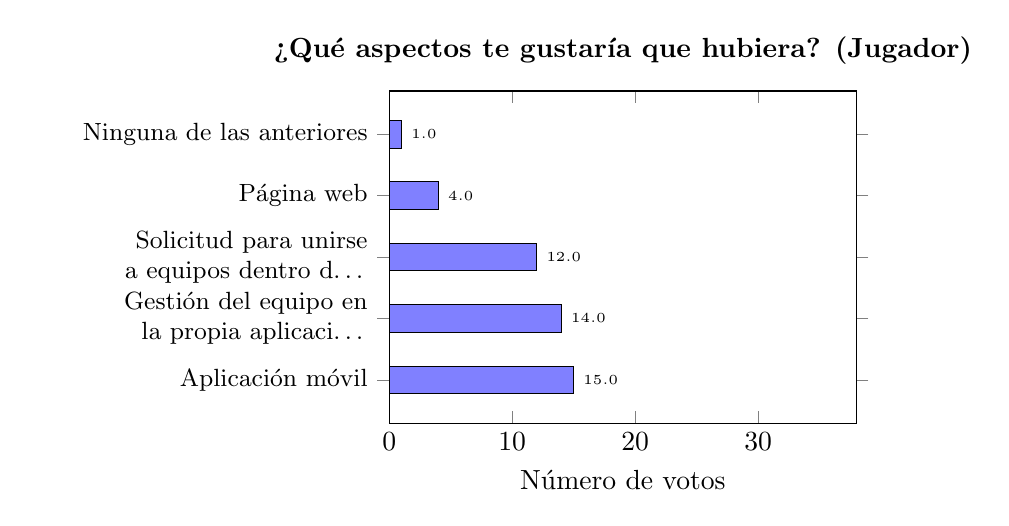
\begin{tikzpicture}
        \begin{axis}[
            title={\textbf{¿Qué aspectos te gustaría que hubiera? (Jugador)}},
            width=0.62*\textwidth,
            xbar,
            bar width=10pt,
            y=0.78cm,
            enlarge y limits={abs=0.55cm},
            xmin=0, xmax=38,
            xlabel={Número de votos},
            ytick={1,2,3,4,5},
            yticklabels={{Aplicación móvil}, {Gestión del equipo en la propia aplicaci\dots}, {Solicitud para unirse a equipos dentro d\dots}, {Página web}, {Ninguna de las anteriores}},
            yticklabel style={
                text width=4.2cm,
                align=right,
                font=\small
            },
            nodes near coords, 
            nodes near coords align={horizontal},
            every node near coord/.append style={
                font=\tiny,
                anchor=west,
                /pgf/number format/.cd, fixed, fixed zerofill, precision=1
            }
        ]
        \addplot[fill=blue!50] coordinates {
            (15, 1) (14, 2) (12, 3) (4, 4) (1, 5)
        };
        \end{axis}
    \end{tikzpicture}
    \label{fig:col_desired_functionalities_player}
    \caption{Nuevas funcionalidades: Jugador}
\end{figure}


Por último, tanto los capitanes como los jugadores buscan una mayor interacción con el sistema a la hora de gestionar los equipos.